\section{Euler Fixes Everything: The Calculus Wars End in a Humiliating Defeat (1730 - 1760)}  

By the time \textbf{Leonhard Euler} came onto the scene, the calculus community was at war. The Newtonians and the Leibnizians weren’t just debating notation—they were waging an \textbf{intellectual blood feud}.  

Each side was convinced that their approach was \textbf{the} correct one. Newton’s camp insisted that calculus should be all about \textbf{fluxions}—because, apparently, describing motion in terms of mystical "flowing quantities" made perfect sense. Meanwhile, Leibniz’s followers swore by \textbf{infinitesimals}, because why not treat change as a weird fraction of an infinitely small number?  

This wasn’t just an argument—it was a full-blown academic street fight. Mathematicians picked sides. The British stuck with Newton. The Continental Europeans rallied behind Leibniz. Papers were written. Insults were exchanged. Careers were ruined. \textbf{Nobody was solving real problems anymore—they were too busy dunking on each other.}  

And then came \textbf{Euler}, who took one look at both sides and basically said:  

\begin{quote}
    \textbf{"You're both wrong. Your notation is terrible. I'm fixing it."}
\end{quote}  

\subsection{Newton’s Fluxions: Good for Motion, Bad for Literally Everything Else}  

Newton’s approach was great—if you were only ever solving physics problems. He thought of \textbf{fluxions} as rates of change over time, writing them as:

\[
\dot{x}, \quad \ddot{x}, \quad \sum o
\]

The problem?  

\begin{itemize}
    \item The dot notation was fine for \textbf{velocity and acceleration}, but completely fell apart when applied to anything outside of physics.
    \item It didn’t extend well to \textbf{functions of multiple variables} (good luck differentiating anything with two inputs).
    \item If you wanted higher derivatives, you were stuck stacking dots like some kind of deranged Morse code.  
\end{itemize}

\subsection{Leibniz’s Infinitesimals: Algebraic, But Still a Mess}  

Leibniz, at least, tried to make calculus \textbf{more symbolic}. His notation,  

\[
dy = \frac{dx}{dx} dy
\]

had some major advantages:

\begin{itemize}
    \item It was \textbf{better for algebra}—you could manipulate differentials like fractions.
    \item It made calculus more \textbf{generalizable}, helping it evolve beyond just motion problems.
\end{itemize}

But let’s not give Leibniz too much credit. His notation still got \textbf{clunky} when dealing with complex equations, and \textbf{nobody really knew what infinitesimals actually were.} Were they numbers? Were they just really, really small? Were they some kind of mathematical hallucination? The debate went unresolved for centuries.

\subsection{Euler Arrives: The Absolute Chad of Notation}  

Euler, being the mathematical powerhouse that he was, looked at the battlefield and decided it was time to \textbf{take out the trash}. He introduced a \textbf{consistent, structured notation} that made calculus readable, logical, and actually useful outside of academic slap fights.

\[
f(x) = x^2 + 3x + 5
\]

Euler’s notation had several advantages:

\begin{itemize}
    \item \textbf{Systematic:} Instead of vague symbols and dots, every function was clearly defined with \( f(x) \).  
    \item \textbf{Extendable:} Higher derivatives were easy to write: \( f^{(n)}(x) \). No more playing \textbf{Guess the Meaning of the Extra Dot.}  
    \item \textbf{Algebra-Friendly:} Differentiation and integration were now \textbf{manipulable equations} instead of mystical processes.  
    \item \textbf{Universally Applicable:} Euler’s system wasn’t just for motion—it worked in \textbf{physics, economics, engineering, and beyond.}  
\end{itemize}

\subsection{Comparing the Three: A Notation War Table}  

\begin{center}
\renewcommand{\arraystretch}{1.5}
\begin{tabular}{|c|c|c|}
\hline
\textbf{Mathematician} & \textbf{Function Notation} & \textbf{Derivative Notation} \\ \hline
Newton & $x$ & $\dot{x}, \ddot{x}$ (Fluxions) \\ \hline
Leibniz & $y$ & $\frac{dy}{dx}$ (Infinitesimals) \\ \hline
Euler & $f(x)$ & $f'(x)$ (The Chad of Notation) \\ \hline
\end{tabular}
\end{center}

\subsection{Euler’s Ultimate Power Move: The Unification of Calculus}  

Euler wasn’t just fixing notation—he was \textbf{rewriting how calculus worked}. His approach was so clean that by the 18th century, \textbf{everyone outside of Britain had abandoned Newton’s fluxions} and switched to Euler’s system.  

This wasn’t just a win—it was a total humiliation. The Newton-Leibniz war had raged for decades, and Euler ended it not with politics, but with a single, brilliant theorem.

\vspace{1em}
\subsubsection{The Euler–Maclaurin Formula: Sums Become Integrals}

In Euler’s time, summation and integration were seen as different beasts:

\begin{itemize}
  \item Sums were discrete: useful for approximating series or solving difference equations.
  \item Integrals were continuous: representing flowing quantities like area or mass.
\end{itemize}

But Euler saw through the illusion. He and Colin Maclaurin derived a formula that let you pass from one to the other:

\[
\sum_{k=a}^{b} f(k) \approx \int_a^b f(x) \, dx + \frac{f(a) + f(b)}{2} + \text{correction terms}
\]

Those “correction terms” involved derivatives of \( f \) and the mysterious **Bernoulli numbers**, which Euler explored obsessively. The full expression was:

\[
\sum_{k=a}^{b} f(k) = \int_a^b f(x)\,dx + \frac{f(a) + f(b)}{2} + \sum_{n=1}^{p} \frac{B_{2n}}{(2n)!} \left(f^{(2n-1)}(b) - f^{(2n-1)}(a)\right) + R_p
\]

This wasn’t just an approximation—it was a revelation. Euler had shown that:

\begin{quote}
\textit{A sum is nothing more than an integral in disguise, plus some curvature.}
\end{quote}

It was the first real unification of the discrete and continuous. No epsilon-deltas. No limits. Just clever algebra and infinite series.

\subsubsection{Why This Was So Powerful}

Euler’s insight allowed mathematicians to:

\begin{itemize}
  \item Estimate large sums using integrals.
  \item Estimate definite integrals using known sums.
  \item Build bridges between algebra and geometry.
\end{itemize}

In practical terms, it let astronomers, engineers, and physicists jump between tables of numbers and flowing systems—without ever needing a rigorous theory of limits.

And he did all this without ever hearing the word “Riemann.”

\vspace{1em}
\subsubsection{Euler’s Diagram: Tangents and Curves}

\begin{center}
\begin{tikzpicture}[scale=1.0]
    
    % Axes
    \draw[->] (-2.5, 0) -- (2.5, 0) node[right] {\small $x$};
    \draw[->] (0, -1) -- (0, 2.5) node[above] {\small $y$};

    % Function f(x)
    \draw[thick, blue] plot[domain=-2:2, smooth] (\x, {0.6*(\x*\x - 2*\x + 1)}) 
        node[right] {\small $f(x) = x^2 - 2x + 1$};

    % Tangent line (Derivative of f(x))
    \draw[dashed, red] (-1.5, -1) -- (2,1.8) 
        node[above] {\small $f'(x) = 2x - 2$};

\end{tikzpicture}
\end{center}

This kind of curve, and its tangent, were Euler’s primary tools. He didn’t need “analysis” to make it work—he needed insight, pattern recognition, and the courage to manipulate infinity.

\begin{quote}
\textbf{Euler didn’t wait for rigour. He made the world computable first—and let the purists catch up later.}
\end{quote}


\subsection{From Intuition to Inertia: Euler Formalizes Galileo's Hunches}

Euler didn’t stop at fixing notation. He looked at physics—the way objects move, spin, and resist motion—and asked the question that made him the legend we know today:

\begin{quote}
\textbf{“What if we actually did the math?”}
\end{quote}

One of the places where this mindset really shined was in the study of \textbf{rotation}—specifically, the concept of \textbf{moment of inertia}.


\begin{figure}[H]
\centering
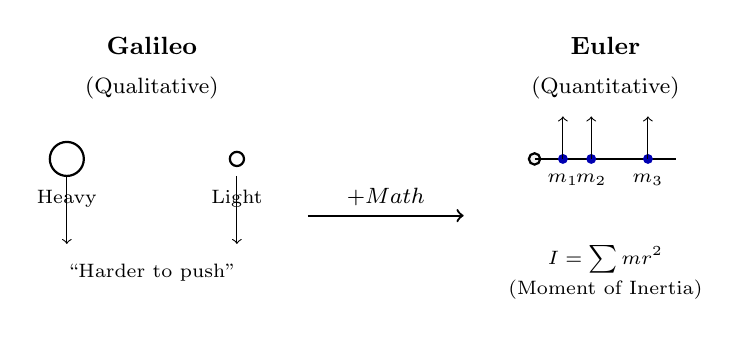
\begin{tikzpicture}[scale=1.8, every node/.style={font=\small}]

  % Left side: Galileo's intuition
  \node[align=center] at (0,2.8) {\textbf{Galileo}};
  \node at (0,2.5) {\footnotesize (Qualitative)};
  \draw[thick] (-0.6,2.0) circle (0.12);
  \draw[thick] (0.6,2.0) circle (0.05);
  \node[below] at (-0.6,1.85) {\scriptsize Heavy};
  \node[below] at (0.6,1.85) {\scriptsize Light};
  \draw[->] (-0.6,1.88) -- (-0.6,1.4);
  \draw[->] (0.6,1.88) -- (0.6,1.4);
  \node at (0,1.2) {\scriptsize “Harder to push”};

  % Arrow from intuition to math
  \draw[->, thick] (1.1,1.6) -- (2.2,1.6);
  \node[above] at (1.65,1.6) {\footnotesize $\text{+ Math}$};

  % Right side: Euler’s formalism
  \node[align=center] at (3.2,2.8) {\textbf{Euler}};
  \node at (3.2,2.5) {\footnotesize (Quantitative)};
  \draw[thick, fill=gray!10] (2.7,2.0) circle (0.04);
  \draw[thick] (2.7,2.0) -- (3.7,2.0);

  % Masses along the rod
  \foreach \x/\label in {2.9/m_1, 3.1/m_2, 3.5/m_3} {
    \fill[blue!70!black] (\x,2.0) circle (0.035);
    \node[below=2pt] at (\x,2.0) {\scriptsize $\label$};
    \draw[->, thin] (\x,2.0) -- (\x,2.3);
  }

  % Label for I = sum m r^2
  \node[align=center] at (3.2,1.2) {
    \scriptsize $I = \sum m r^2$ \\
    \scriptsize (Moment of Inertia)
  };

\end{tikzpicture}
\caption{Galileo knew heavier objects were harder to move. Euler turned that intuition into math — introducing the moment of inertia $I = \sum m r^2$, quantifying rotational resistance.}
\end{figure}



\subsubsection{Galileo’s Gut Feeling}

Before Euler came along with his calculus war cleanup crew, Galileo had already been exploring how objects move. He had a brilliant physical intuition and could describe how bodies accelerated, rolled, or fell. 

But Galileo's take on rotational motion was still pretty fuzzy. He understood that spinning objects seemed to resist changes in their spin, and that mass and distance from the axis mattered somehow—but his explanations were mostly qualitative. He talked about "heaviness of rotation" without formalizing what that actually meant.

He knew something was happening, but he couldn’t quite bottle it up in an equation.


\begin{figure}[H]
\centering
\begin{tikzpicture}[scale=2.5, every node/.style={font=\small}]

  % Wheel (circle)
  \draw[thick] (0,0) circle (1);

  % Central axis
  \fill[black] (0,0) circle (0.03);
  \node[below right=2pt] at (0,0) {Axis};

  % Mass points around the edge
  \foreach \angle in {0, 90, 180, 270} {
    \coordinate (P) at ({cos(\angle)}, {sin(\angle)});
    \fill[blue] (P) circle (0.05);
    \node at ($(P)+(0.2,0.1)$) {\scriptsize Mass};
  }

  % Arrows indicating rotation
  \draw[->, thick, red!60!black] (1.1,0) arc[start angle=0, end angle=90, radius=1.1];
  \node[red!60!black] at (0.8,0.7) {\scriptsize Spinning};

  % Question mark to indicate qualitative feel
  \node at (-1.1,-0.8) {\Large \textbf{?}};
  \node[align=center] at (0,-1.2) {
    \scriptsize ``Heaviness of rotation'' \\
    \scriptsize (Galileo's intuition)
  };

\end{tikzpicture}
\caption{Galileo sensed that mass and distance from the axis affected rotation, but lacked the tools to formalize it. His intuition hinted at what Euler would later define as moment of inertia.}
\end{figure}



\subsubsection{Euler’s Turn: Defining Rotational Resistance}

Euler stepped in and gave that "heaviness of rotation" a name—and more importantly, a formula.

\[
I = \sum m r^2
\]

Where:
\begin{itemize}
    \item \( I \) is the \textbf{moment of inertia}
    \item \( m \) is the mass of a point in the object
    \item \( r \) is the distance from that point to the axis of rotation
\end{itemize}

In other words: the farther mass is from the center, the more it resists rotational acceleration. And unlike Galileo, Euler didn’t just say this. He proved it. With math. 

He generalized it, extended it to rigid bodies, and tied it directly into his \textbf{Euler’s Laws of Motion}—a rotational analog to Newton’s laws. It wasn’t just about mass anymore; it was about how that mass was distributed. This was the foundation of \textbf{rotational dynamics} as we know it today.


\begin{figure}[H]
\centering
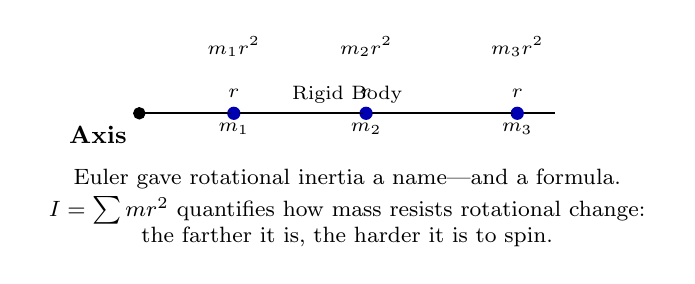
\begin{tikzpicture}[scale=2.4, every node/.style={font=\small}]

  % Axis of rotation
  \filldraw[black] (0,0) circle (0.03);
  \node[below left=1pt] at (0,0) {\textbf{Axis}};

  % Rod or body
  \draw[thick] (0,0) -- (2.2,0);
  \node[above] at (1.1,0) {\scriptsize Rigid Body};

  % Point masses and radius vectors
  \foreach \x/\mass in {0.5/m_1, 1.2/m_2, 2.0/m_3} {
    \fill[blue!70!black] (\x,0) circle (0.035);
    \draw[dashed] (0,0) -- (\x,0);
    \node[below] at (\x,0) {\scriptsize $\mass$};
    \node[above] at (\x,0.03) {\scriptsize $r$};
    \node[above=10pt] at (\x,0.1) {\scriptsize $\mass r^2$};
  }

  % Moment of inertia label
  \node at (1.1,-0.5) {
    \begin{minipage}{0.65\linewidth}
      \centering
      \footnotesize Euler gave rotational inertia a name—and a formula. \\
      \vspace{2pt}
      $I = \sum m r^2$ quantifies how mass resists rotational change: the farther it is, the harder it is to spin.
    \end{minipage}
  };

\end{tikzpicture}
\caption{Euler defined rotational resistance with the moment of inertia: $I = \sum m r^2$. It’s not just mass—it’s where that mass is placed.}
\end{figure}



\subsubsection{The Controversy: Who Really Deserved the Credit?}

Now, as with all great ideas in science, credit is complicated.

Some argue that Euler didn’t “discover” the moment of inertia so much as refine what Galileo and others had already hinted at. After all, rotational resistance had been observed and described centuries earlier.

But here’s the thing: \textbf{Euler named it}, derived the equations, applied it across multiple physical systems, and baked it directly into his larger mechanical framework. He took a vague physical intuition and turned it into a quantifiable, generalizable tool.

That’s the difference between noticing that spinning things are hard to stop—and building the math that can model a satellite, a spinning top, or a collapsing star.

\subsubsection{The Real Power Move: Abstracting Physics into Calculus}

Euler didn’t just do math. He rewrote physics using math.

He wasn’t content to say “this thing spins weird.” He asked: “How can I describe spinning with the same language I use to describe straight-line motion?”

And he succeeded.

Thanks to Euler:
\begin{itemize}
    \item We can model rotational kinetic energy: \( \frac{1}{2} I \omega^2 \)
    \item We have Euler’s equations of motion for rigid bodies
    \item We can launch spacecraft, design gyroscopes, and simulate 3D physics in video games
\end{itemize}

Galileo laid the philosophical groundwork. Euler built the infrastructure.

\begin{center}
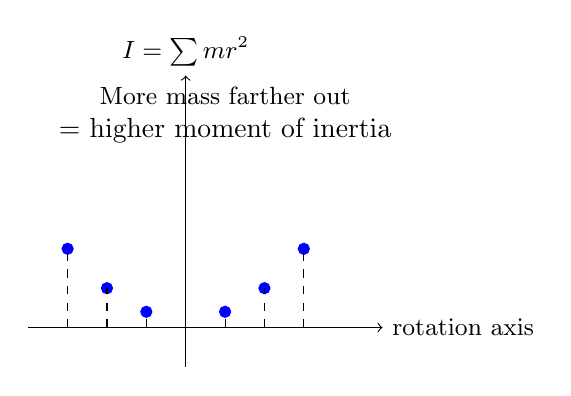
\begin{tikzpicture}[scale=1.0]
    % Axis
    \draw[->] (-2,0) -- (2.5,0) node[right] {\small rotation axis};
    \draw[->] (0,-0.5) -- (0,3.2) node[above] {\small $I = \sum m r^2$};

    % Mass points and distances
    \foreach \x in {-1.5,-1,-0.5,0.5,1,1.5} {
        \filldraw[blue] (\x, {0.1 + 0.4*\x*\x}) circle (2pt);
        \draw[dashed] (\x,0) -- (\x, {0.1 + 0.4*\x*\x});
    }

    \node[align=center] at (0.5, 2.7) {\small More mass farther out \\ = higher moment of inertia};
\end{tikzpicture}
\end{center}

So next time you see something spinning and refusing to stop, thank Galileo for noticing—and Euler for explaining.

\subsection{Euler and Kepler: Rotation Meets the Cosmos}

By the time Euler formalized the concept of \textbf{moment of inertia}, he wasn’t just helping physicists understand spinning tops or flywheels. He was laying the groundwork for a rotational understanding of planetary motion itself—including the insights at the heart of \textbf{Kepler’s Second Law}.

\subsubsection{The Moment of Area: A Rotational Parallel}

Recall Kepler’s Second Law: planets sweep out \textbf{equal areas in equal time}. That’s a statement about how angular motion varies with distance from the Sun. In Newton’s formulation, it’s explained as the consequence of a centripetal force acting through a central point—gravity tugging inward, and angular momentum conserved.

\begin{figure}[H]
\centering
\begin{tikzpicture}[scale=2.5, every node/.style={font=\small}]

  % Central body (Sun)
  \filldraw[yellow!80!orange] (0,0) circle (0.04);
  \node[below right=1pt] at (0,0) {\textbf{Sun}};

  % Orbit path
  \draw[thick,gray!60] (0,0) circle (1.1);

  % Two orbital positions
  \coordinate (A) at ({1.1*cos(30)}, {1.1*sin(30)});
  \coordinate (B) at ({1.1*cos(110)}, {1.1*sin(110)});
  \filldraw[blue] (A) circle (0.02);
  \filldraw[blue] (B) circle (0.02);

  \node[right=2pt] at (A) {\scriptsize Position 1};
  \node[left=2pt] at (B) {\scriptsize Position 2};

  % Central force vectors (gravity)
  \draw[->, thick, red!70!black] (A) -- ($(A)!0.3!(0,0)$);
  \draw[->, thick, red!70!black] (B) -- ($(B)!0.3!(0,0)$);

  \node at ($(A)!0.5!(0,0)+(0.05,-0.05)$) {\scriptsize $\vec{F}_{\text{gravity}}$};
  \node at ($(B)!0.5!(0,0)+(-0.1,0.05)$) {\scriptsize $\vec{F}_{\text{gravity}}$};

  % Equal area sweeps
  \fill[blue!20, opacity=0.4] (0,0) -- (A) arc[start angle=30, end angle=60, radius=1.1] -- cycle;
  \fill[blue!20, opacity=0.4] (0,0) -- (B) arc[start angle=110, end angle=140, radius=1.1] -- cycle;

  \node at (0.3,0.4) {\scriptsize Equal areas};

  % Caption
  \node at (0,-1) {
    \begin{minipage}{0.75\linewidth}
      \centering
      \footnotesize
      Newton explained Kepler’s Second Law through a central force: gravity pulls inward at all times, keeping the planet in orbit and ensuring that equal areas are swept out in equal time. The symmetry comes from the center—not rotation, but radial force.
    \end{minipage}
  };

\end{tikzpicture}
\caption{Newton’s interpretation of Kepler’s Second Law: planets sweep equal areas because of a centripetal force (gravity) acting through a fixed point—the Sun. The force is always radial, not rotational.}
\end{figure}


But Euler’s lens adds another twist:

\begin{quote}
What if the key quantity isn’t just area, or force—but how hard it is to \textit{change} the planet’s motion at any given radius?
\end{quote}

Enter the moment of inertia:

\[
I = \sum m r^2 \quad \Rightarrow \quad \text{or for continuous systems: } I = \int r^2 \, dm
\]

While Kepler was talking about sweeping areas, Euler would have looked at the \textbf{resistance to changing that sweep}—how much torque would be required to alter a planet’s path.


\begin{figure}[H]
\centering
\begin{tikzpicture}[scale=2.5, every node/.style={font=\small}]

  % Central mass (e.g., Sun)
  \filldraw[yellow!80!orange] (0,0) circle (0.04);
  \node[below right=1pt] at (0,0) {\textbf{Sun}};

  % Orbit ellipse (for simplicity, circle)
  \draw[thick,gray!60] (0,0) circle (1.1);

  % Two positions: closer and farther
  \coordinate (A) at ({1.1*cos(30)}, {1.1*sin(30)});
  \coordinate (B) at ({1.1*cos(120)}, {1.1*sin(120)});
  \filldraw[blue] (A) circle (0.02);
  \filldraw[blue] (B) circle (0.02);

  \node[right=2pt] at (A) {\scriptsize Position 1};
  \node[left=2pt] at (B) {\scriptsize Position 2};

  % Sector areas for equal time sweep
  \fill[blue!15, opacity=0.5] (0,0) -- (A) arc[start angle=30, end angle=60, radius=1.1] -- cycle;
  \fill[blue!15, opacity=0.5] (0,0) -- (B) arc[start angle=120, end angle=150, radius=1.1] -- cycle;

  \node at (0.5,0.4) {\scriptsize Equal areas};

  % Radius vectors
  \draw[->, thick] (0,0) -- (A);
  \draw[->, thick] (0,0) -- (B);

  \node at (0.3,0.85) {\scriptsize $r_1$};
  \node at (-0.8,0.6) {\scriptsize $r_2$};

  % Small mass elements at each position
  \draw[->, red!70!black, thick] (A) -- ++(60:0.3);
  \draw[->, red!70!black, thick] (B) -- ++(150:0.3);
  \node[red!70!black] at ($(A)+(60:0.3)+(0.15,0)$) {\scriptsize $m r_1^2$};
  \node[red!70!black] at ($(B)+(150:0.3)+(-0.2,0)$) {\scriptsize $m r_2^2$};

  % Label
  \node at (0,-1.0) {
    \begin{minipage}{0.75\linewidth}
      \centering
      \footnotesize Kepler said planets sweep out equal areas in equal time. Euler extended this thinking by introducing the moment of inertia: a measure of how hard it is to change that angular motion. The farther the mass is from the center, the more it resists — not linearly, but quadratically, as $I = \sum m r^2$.
    \end{minipage}
  };

\end{tikzpicture}
\caption{Kepler described how planets sweep equal areas in equal time. Euler’s moment of inertia added a deeper rotational insight: resistance to changing that sweep grows with $r^2$.}
\end{figure}



\subsubsection{From Kepler to Angular Momentum}

Using modern notation, Kepler’s Second Law implies conservation of angular momentum:

\[
L = I \omega = \text{constant}
\]

Where:
\begin{itemize}
    \item \( I = m r^2 \) is the moment of inertia (for a point mass),
    \item \( \omega = \frac{d\theta}{dt} \) is angular velocity,
    \item \( L \) is the angular momentum.
\end{itemize}

\begin{figure}[H]
\centering
\begin{tikzpicture}[scale=2.5, every node/.style={font=\small}]

  % Central body (e.g., Sun)
  \filldraw[yellow!80!orange] (0,0) circle (0.04);
  \node[below right=1pt] at (0,0) {\textbf{Sun}};

  % Orbit path (circular)
  \draw[thick,gray!60] (0,0) circle (1.1);

  % Planet position
  \coordinate (P) at ({1.1*cos(60)}, {1.1*sin(60)});
  \filldraw[blue] (P) circle (0.02);
  \node[above right=1pt] at (P) {Planet};

  % Radius vector r
  \draw[->, thick] (0,0) -- (P) node[midway, above left] {\scriptsize $r$};

  % Angular velocity arc
  \draw[->, thick,blue!60!black] (0.7,0) arc[start angle=0,end angle=60,radius=0.7];
  \node at (0.8,0.35) {\scriptsize $\omega = \frac{d\theta}{dt}$};

  % Angular momentum vector (perpendicular)
  \draw[->, thick,red!70!black] (P) -- ++(150:0.4);
  \node[red!70!black] at ($(P)+(150:0.45)$) {\scriptsize $L = I\omega$};

  % Inertia label
  \node at (-1.2,-0.7) {
    \begin{minipage}{0.7\linewidth}
      \centering
      \footnotesize Kepler’s equal-area law implies conservation of angular momentum. With $I = m r^2$ and $\omega = \frac{d\theta}{dt}$, we get $L = I\omega$, which stays constant as the planet orbits.
    \end{minipage}
  };

\end{tikzpicture}
\caption{Kepler's Second Law implies angular momentum is conserved: $L = I\omega = m r^2 \cdot \frac{d\theta}{dt}$. As the planet moves, $r$ and $\omega$ may change—but their product $L$ remains constant.}
\end{figure}


From this, we can derive Kepler’s area law:

\[
\frac{dA}{dt} = \frac{1}{2} r^2 \frac{d\theta}{dt} = \frac{L}{2m}
\]

This means:
- When the planet is closer to the Sun (\( r \) is small), \( \omega \) must be large.
- When it's farther away, it rotates more slowly.
- But in both cases, the \textbf{area swept per unit time stays constant}.

Kepler saw the geometry.  
Leibniz wrote the integral.  
Newton explained the force.  
\textbf{Euler explained the resistance.}


\begin{figure}[H]
\centering
\begin{tikzpicture}[scale=2.5, every node/.style={font=\small}]

  % Central body
  \filldraw[yellow!80!orange] (0,0) circle (0.04);
  \node[below right=1pt] at (0,0) {\textbf{Sun}};

  % Orbit path (circular)
  \draw[thick,gray!60] (0,0) circle (1.1);

  % Two positions: close and far
  \coordinate (P1) at ({1.1*cos(30)}, {1.1*sin(30)});
  \coordinate (P2) at ({1.1*cos(150)}, {1.1*sin(150)});
  \filldraw[blue] (P1) circle (0.02);
  \filldraw[blue] (P2) circle (0.02);
  \node[right=2pt] at (P1) {\scriptsize Closer};
  \node[left=2pt] at (P2) {\scriptsize Farther};

  % Radius vectors
  \draw[->, thick] (0,0) -- (P1) node[midway, above right] {\scriptsize $r_1$};
  \draw[->, thick] (0,0) -- (P2) node[midway, above left] {\scriptsize $r_2$};

  % Angular velocity arrows
  \draw[->, red!70!black, thick] (P1) -- ++(120:0.3);
  \draw[->, red!70!black, thick] (P2) -- ++(210:0.15);
  \node[red!70!black] at ($(P1)+(120:0.35)$) {\scriptsize $\omega_1$ (fast)};
  \node[red!70!black] at ($(P2)+(210:0.35)$) {\scriptsize $\omega_2$ (slow)};

  % Equal area sectors
  \fill[blue!15, opacity=0.4] (0,0) -- (P1) arc[start angle=30, end angle=50, radius=1.1] -- cycle;
  \fill[blue!15, opacity=0.4] (0,0) -- (P2) arc[start angle=150, end angle=170, radius=1.1] -- cycle;

  \node at (0.2,0.3) {\scriptsize Equal areas swept};

  % Label
  \node at (0,-1.0) {
    \begin{minipage}{0.75\linewidth}
      \centering
      \footnotesize Kepler’s area law in modern form: $\displaystyle \frac{dA}{dt} = \frac{1}{2}r^2 \frac{d\theta}{dt} = \frac{L}{2m}$. \\
      Planets move faster when closer, slower when farther, but always sweep equal areas in equal time.
    \end{minipage}
  };

\end{tikzpicture}
\caption{Kepler’s Second Law as a statement of conserved angular momentum: $\frac{dA}{dt} = \frac{1}{2}r^2 \omega = \frac{L}{2m}$. The geometry hides a deep rotational symmetry.}
\end{figure}


\subsubsection{Why Euler's View Matters}

Euler didn’t reinterpret Kepler—he reinforced it by clarifying \textbf{what stays constant (angular momentum)} and \textbf{why}.

Unlike Newton’s triangles or Leibniz’s infinitesimals, Euler’s framework makes it clear that:
- Planetary motion isn’t just conserved geometrically or algebraically—it’s dynamically constrained by how mass behaves under rotation.
- This opens the door to generalizations: spinning tops, precessing orbits, gyroscopes, and eventually, relativity.

\subsubsection*{Diagram: Angular Momentum and Sweeping Areas}

\begin{figure}[H]
\centering
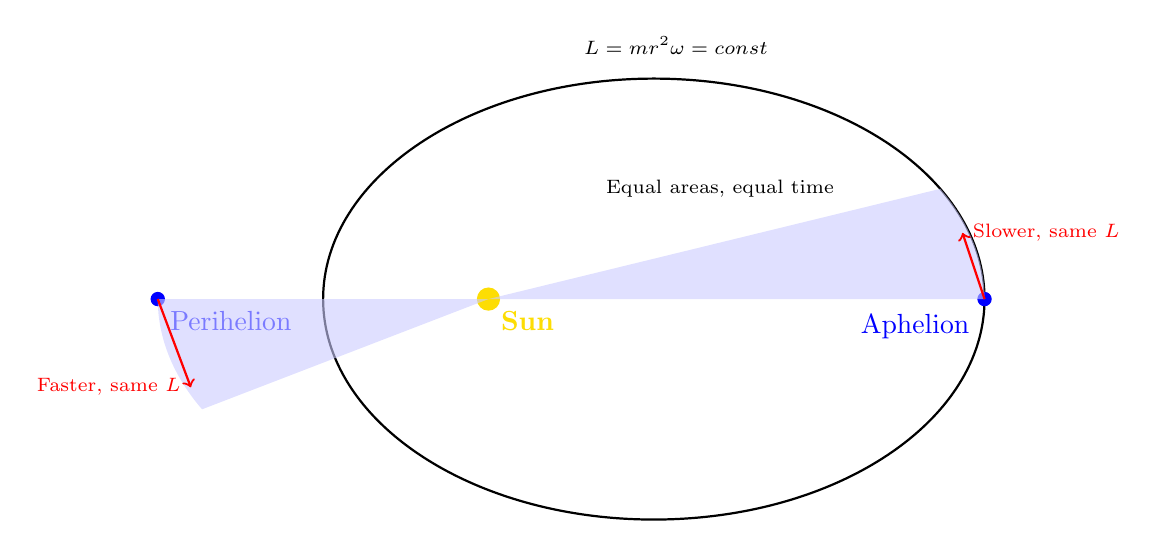
\begin{tikzpicture}[scale=2.8]
  % Elliptical orbit
  \draw[thick] (0,0) ellipse (1.5 and 1);

  % Sun at one focus
  \filldraw[yellow!80!orange] (-0.75,0) circle (0.05) node[below right=1pt] {\textbf{Sun}};

  % Aphelion and Perihelion
  \filldraw[blue] (1.5,0) circle (0.03) node[below left=2pt] {Aphelion};
  \filldraw[blue] (-2.25,0) circle (0.03) node[below right=1pt] {Perihelion};

  % Wedges for equal areas
  \fill[blue!20, opacity=0.6] 
    (-0.75,0) -- (1.5,0) arc[start angle=0,end angle=30,x radius=1.5cm, y radius=1cm] -- cycle;

  \fill[blue!20, opacity=0.6] 
    (-0.75,0) -- (-2.25,0) arc[start angle=180,end angle=210,x radius=1.5cm, y radius=1cm] -- cycle;

  % Angular momentum vectors
  \draw[->, red, thick] (1.5,0) -- (1.4,0.3) node[right] {\scriptsize Slower, same $L$};
  \draw[->, red, thick] (-2.25,0) -- (-2.1,-0.4) node[left] {\scriptsize Faster, same $L$};

  % Equation annotation
  \node at (0.1,1.15) {\scriptsize $L = m r^2 \omega = \text{const}$};

  % Label
  \node at (0.3,0.5) {\scriptsize Equal areas, equal time};

\end{tikzpicture}
\caption{Euler’s lens on Kepler’s law: Equal areas imply constant angular momentum, linking rotational inertia to orbital dynamics.}
\end{figure}

\subsubsection{The Chain of Insight}

\begin{center}
\begin{tikzpicture}[node distance=1.5cm and 2.8cm, every node/.style={align=center}]
\node (kepler) {\textbf{Kepler} \\ Geometry of Areas};
\node (leibniz) [below left=of kepler] {\textbf{Leibniz} \\ Infinitesimal Integrals};
\node (newton) [below right=of kepler] {\textbf{Newton} \\ Central Force, Geometry};
\node (euler) [below=of kepler] {\textbf{Euler} \\ Angular Momentum and Inertia};

\draw[->] (kepler) -- (leibniz);
\draw[->] (kepler) -- (newton);
\draw[->] (leibniz) -- (euler);
\draw[->] (newton) -- (euler);
\end{tikzpicture}
\end{center}

\begin{quote}
\textit{Kepler measured the sky. Newton explained the forces. Leibniz wrote the math. Euler made it move.}
\end{quote}





\subsection{Kepler’s Second Law: Who Did What, and Why Euler Wins Anyway}

Now that the calculus wars have cooled and the concept of rotational inertia is on the table, we can revisit the idea that started all of this: \textbf{Kepler’s Second Law} — the law that says a planet sweeps out equal areas in equal times.

This elegant geometric principle became a lens through which Newton, Leibniz, and Euler each interpreted motion — each in radically different ways. And the way they did it reflects how they saw the universe.

\subsubsection*{Newton: Geometry in the Service of Force}

In the \textit{Principia}, Newton didn’t use algebra or calculus to explain Kepler’s Second Law. He went full Euclid.

He imagined a planet moving in discrete steps — tracing a piecewise linear orbit. At each instant, it moved in a straight line, then was pulled slightly toward the sun. These repeated deflections formed triangular wedges. He showed that:

\begin{quote}
If a planet sweeps out equal areas in equal times, then the force acting on it must always point toward the center.
\end{quote}

And he proved the converse: if the force is always directed toward a center (a central force), then the planet must sweep out equal areas in equal times.

\textbf{Newton’s notation:}
\begin{itemize}
    \item No \( r \) or \( \theta \)
    \item No \( \frac{dA}{dt} \)
    \item Just geometry, lines, triangles, proportions, and ratios.
\end{itemize}

His insight was physical, but his method was classical.

\textbf{Key Contribution:}
\begin{itemize}
    \item \textbf{Equal areas} \(\Rightarrow\) \textbf{Central force}
    \item \textbf{Central force} \(\Rightarrow\) \textbf{Equal areas}
\end{itemize}

\subsubsection*{Leibniz: Algebra in the Service of Accumulation}

Leibniz never directly addressed Kepler’s laws, but he invented something that would become essential: a language for infinitesimal change. Where Newton used triangles, Leibniz used differentials.

For Leibniz, motion was not geometric but algebraic — not drawn, but summed. He introduced symbols like:

\[
dx, \quad dy, \quad \int
\]

Even though he never wrote down an equation for area swept over time, the concept of summing infinitely small pieces — infinitesimal arcs, infinitesimal times — was baked into his calculus.

He might have imagined area as accumulating via:

\[
dA = \text{(something)} \cdot dt
\]

Though the modern form using radius and angle came later, Leibniz laid the foundation. He thought not in terms of curves on a page, but quantities in symbolic motion — each differential a whisper of change.

\textbf{Key Contribution:}
\begin{itemize}
    \item Provided a symbolic system for expressing infinitesimal change
    \item Created the tools needed to reinterpret Kepler’s geometry as algebra
\end{itemize}

\subsubsection*{Euler: The Synthesis — Motion, Resistance, and Invariance}

Euler entered the scene armed with Newton’s physics, Leibniz’s calculus, and his own uncanny ability to see structure in motion. Where Newton had relied on geometry and Leibniz had crafted a symbolic language of differentials, Euler fused the two into a coherent analytical mechanics.

He did not use modern vector notation or partial derivatives. Instead, he worked with differentials and algebraic expressions of motion, writing things like:

\[
dz = M\,dx + N\,dy
\]

and thinking of \( M \) and \( N \) as expressions of how a quantity changed with respect to \( x \) and \( y \) independently — though he wouldn’t call them “partials” as we do today.

For Kepler’s Second Law, Euler understood that the sweeping of area over time implied a relationship between a planet’s distance from the sun and its rotational velocity. He recognized that when the radius to the sun was shorter, the velocity had to be greater to sweep the same area — and vice versa.

Euler interpreted this balance as a kind of conserved quantity, though not yet named “angular momentum.” In his language, this meant:

- The product of distance and rotational speed must remain constant
- The accumulation of small sectors (areas) over time must proceed at a uniform rate

He may have written:

\[
\text{Let } dA \text{ be the differential area swept, and } t \text{ the time, then } \frac{dA}{dt} = \text{constant}
\]

But Euler would not have broken this into \( r^2 \frac{d\theta}{dt} \) — polar coordinates were not fully formalized yet.

\textbf{What Euler contributed:}
\begin{itemize}
    \item Treated area sweep as a continuous accumulation of differentials in time
    \item Identified the conservation principle implicit in Kepler’s law
    \item Created a language to analyze motion via functions of multiple changing quantities (time, distance, angle), without modern coordinate systems
\end{itemize}

Euler's genius was not in introducing new physical laws — but in giving existing ones a form that could be used, manipulated, and generalized. His work didn’t just preserve Kepler’s Second Law — it made it calculable.

\subsubsection*{From Geometry to Polar Coordinates: The Path to Modern Notation}

The expressions we now associate with Kepler’s Second Law — like:

\[
\frac{dA}{dt} = \frac{1}{2} r^2 \frac{d\theta}{dt}
\]

— were not written by Kepler, Newton, Leibniz, or even Euler. They emerged in the later 18th and early 19th centuries, as the **polar coordinate system** was formalized by mathematicians such as **Gregory**, **Bernoulli**, and **Euler himself** in related contexts.

In polar coordinates, a point’s position is defined by:

\[
(r, \theta)
\]

Where:
- \( r \) is the distance from a central origin (e.g., the sun)
- \( \theta \) is the angle from a fixed axis

With this system, the area swept out by a moving object over time could be written as:

\[
\frac{dA}{dt} = \frac{1}{2} r^2 \frac{d\theta}{dt}
\]

This formula unifies:
- Geometry (via area)
- Motion (via \( \frac{d\theta}{dt} \))
- Position (via \( r \))

And ultimately leads to a modern interpretation of Kepler’s Second Law as the conservation of angular momentum:

\[
L = m r^2 \frac{d\theta}{dt}
\]

But this leap required the mathematical infrastructure that Euler helped lay, even if he did not yet write with these symbols.

\textbf{Why Polar Coordinates Mattered:}
\begin{itemize}
    \item Translated classical geometric motion into symbolic calculus
    \item Allowed explicit computation of area sweep rates
    \item Enabled the unification of Kepler’s laws with Newtonian mechanics and conservation principles
\end{itemize}

In short, polar coordinates turned Euler’s insights into tools — and gave future physicists the power to simulate the sky with a pen.



\subsubsection*{Final Scorecard: Who Did What?}

\begin{center}
\renewcommand{\arraystretch}{1.6}
\begin{tabular}{|c|p{4.5cm}|p{6.5cm}|}
\hline
\textbf{Mathematician} & \textbf{What They Saw} & \textbf{What They Contributed} \\ \hline
\textbf{Kepler} & The sky & Planets sweep equal areas in equal time \\ \hline
\textbf{Newton} & Geometry in motion & Equal areas imply central force; proved it with classical constructions \\ \hline
\textbf{Leibniz} & Infinitesimal change & Introduced calculus as a symbolic method for accumulation \\ \hline
\textbf{Euler} & Invariance in motion & Interpreted Kepler's law as angular momentum conservation; bridged geometry and dynamics \\ \hline
\end{tabular}
\end{center}

\begin{quote}
\textit{Newton showed the force. Leibniz wrote the language. Euler unified the laws.}
\end{quote}

\subsubsection*{Diagram: One Law, Three Interpretations}

\begin{figure}[H]
\centering
\begin{tikzpicture}[node distance=1.4cm and 3.2cm, every node/.style={align=center}]
\node (kepler) {\textbf{Kepler} \\ Area swept = constant};
\node (newton) [below left=of kepler] {\textbf{Newton} \\ Geometry and force};
\node (leibniz) [below right=of kepler] {\textbf{Leibniz} \\ Symbolic accumulation};
\node (euler) [below=of kepler] {\textbf{Euler} \\ Angular momentum conserved};

\draw[->] (kepler) -- (newton);
\draw[->] (kepler) -- (leibniz);
\draw[->] (newton) -- (euler);
\draw[->] (leibniz) -- (euler);
\end{tikzpicture}
\caption{Kepler saw the pattern. Newton proved the force. Leibniz wrote the symbols. Euler explained the physics.}
\end{figure}


